\documentclass[a4paper,12pt,twoside]{article}

\usepackage{amsmath}
%\usepackage{cite}
\usepackage[hidelinks]{hyperref}
\usepackage[includeheadfoot,margin=30mm]{geometry}
\usepackage{subcaption}
\usepackage{graphicx}
\usepackage{booktabs}
\usepackage{multirow}
\usepackage{siunitx}
\usepackage{natbib}
\usepackage{url}
\usepackage[english]{babel}
\usepackage{blindtext}

\usepackage{fancyhdr}
\pagestyle{fancy}
\fancyhf{}
\fancyhead[LE,RO]{\leftmark}
\fancyfoot[CE,CO]{\thepage}


\geometry{left=30mm,right=30mm,top=35mm,bottom=30mm,headheight=15pt}

\graphicspath{{./img/}}


\begin{document}
	
	\begin{titlepage}
		\centering
		\begin{figure}[!h]
			\centering
			
\includegraphics[width=0.5\textwidth]{figures/UZH.png}
		\end{figure}
		\Large{\textbf{Optimal Lookback Window in Time-Series Momentum}\\}

		
		\vfill
		
		\large{\href{mailto:thomas.meier6@uzh.ch}{Thomas Meier} (19-738-400) \\
				\href{mailto:thomas.meier6@uzh.ch}{Ana Jazbinsek} (22-737-753)\\}
		
		\vfill
			
		\large{\today}
		
		\vfill
		\vfill
	
		\large{Department of Banking \& Finance \\ Digital Tools for Finance \\ Dr. Igor Pozdeev\\ }
	
		\vfill
		\begin{abstract}
			Abstract. Lorem ipsum dolor sit amet, consetetur sadipscing elitr, sed diam nonumy eirmod tempor invidunt ut labore et dolore magna aliquyam erat, sed diam voluptua. At vero eos et accusam et justo duo dolores et ea rebum. Stet clita kasd gubergren, no sea takimata sanctus est Lorem ipsum dolor sit amet. Lorem ipsum dolor sit amet, consetetur sadipscing elitr, sed diam nonumy eirmod tempor invidunt ut labore et dolore magna aliquyam erat, sed diam voluptua. At vero eos et accusam et justo duo dolores et ea rebum. Stet clita kasd gubergren, no sea takimata sanctus est Lorem ipsum dolor sit amet.
			
			\vspace{3mm}
			
			\textbf{Keywords:} Value, Momentum, Score, Investment Strategy
		\end{abstract}
		
		
	\end{titlepage}

    \clearpage	
    \thispagestyle{empty}\mbox{}
    \clearpage

	\pagenumbering{roman}
    \setcounter{page}{1}
	\tableofcontents
	
	\clearpage
	\listoffigures
	
	\listoftables
	
	\clearpage
    \pagenumbering{arabic}
    \setcounter{page}{1}
    \setlength{\parindent}{0pt}
    \setlength{\parskip}{8pt}
%---------------------------------------

\section{Introduction}
Cross-sectional momentum strategies, which involve ranking assets based on past performance and constructing portfolios that long top performers while shorting underperformers, have been extensively studied in financial literature. The seminal work by \cite{jegadeesh1993returns} demonstrated that such strategies yield significant positive returns in equity markets. Subsequent research has confirmed the robustness of the momentum effect across various asset classes and geographies, challenging the efficient market hypothesis postulated by \cite{fama1970efficient}.
\\~\\
A critical aspect of implementing such momentum strategies is determining the optimal lookback period, e.g. the historical timeframe used to assess past performance. The choice of lookback window significantly influences the strategy's effectiveness, as it affects the identification of genuine performance trends versus short-term anomalies. Studies have explored various lookback periods, ranging from short-term (e.g., 1-3 months) to long-term (e.g., 12 months), to ascertain their impact on returns. While \cite{jegadeesh1993returns} found significant outperformance for momentum strategies between horizons from three to twelve months, they also found evidence of a reversal of this trend at longer horizons in the following years. They attribute this reversal effect to overreaction hypotheses similar to bubble dynamics but did not investigate it much further.
Other studies such as \cite{nagel2001overreaction}, investigated specifically this long-term reversal effect of momentum and found that this reversal effect can largely be attributed to predictable book-to-market effects.\footnote{Past winners that outperform significantly decrease their relative B/M ratio compared to peers.} After controlling for this effect, \cite{nagel2001overreaction} finds that momentum seems to persist further.
\\~\\
Given this background, this project aims to examine different lookback periods for a cross-sectional momentum strategy in equity markets. Instead of the traditional 12-1 month momentum portfolios we examine look back windows up to 24 months.
\\~\\
Understanding the implications of different lookback windows is essential for both academics and practitioners aiming to optimize momentum-based investment strategies. This paper contributes to the existing literature by systematically analyzing the performance of cross-sectional momentum strategies across various lookback periods in equity markets, providing insights into their relative effectiveness and guiding the selection of appropriate parameters for portfolio construction.
\newpage
\section{Literature Review}
Momentum investing, a strategy that capitalizes on the persistence of asset price trends, has been a focal point in financial research for decades. The foundational study by \cite{jegadeesh1993returns} unveiled that stocks exhibiting superior returns over a 3- to 12-month period tend to continue outperforming in subsequent months, challenging the efficient market hypothesis. This phenomenon, termed the "momentum effect," has been observed across various asset classes and markets prompting extensive academic inquiry \citep{asness2013value, baltas2013momentum}.

%%%%%%
Over time, researchers have proposed multiple explanations for the momentum effect. Behavioral theories suggest that investor biases, such as delayed overreaction to information, contribute to price continuations. Conversely, risk-based explanations posit that momentum profits are compensation for bearing systematic risks not captured by traditional asset pricing models. Despite these efforts, a consensus on the underlying causes of momentum remains elusive \citep{barberis1998model, grinblatt2005prospect, bikhchandani1992theory}.

Momentum strategies are primarily categorized into two types: cross-sectional and time-series momentum. Cross-sectional momentum, as examined by \cite{jegadeesh1993returns}, involves ranking assets based on relative past performance, going long on top performers and short on underperformers. In contrast, time-series momentum, explored by \cite{moskowitz2012time}, assesses each asset's own past returns, taking positions based on whether past performance was positive or negative. While both strategies aim to exploit trend persistence, they differ in implementation and underlying assumptions.

This paper focuses on cross-sectional momentum strategies, specifically analyzing the impact of varying lookback periods on performance. Prior studies have investigated the influence of different formation and holding periods on momentum returns. For instance, \cite{jegadeesh1993returns} found that strategies with formation periods of 3 to 12 months yielded significant positive returns. However, \cite{nagel2001overreaction} provided some evidence for momentum at even longer horizons. Moreover, the optimal look back window may vary across markets, which necessitates further examination.
\newpage
\section{Dataset}
The project makes use of the Yahoo Finance API, in order to download the desired time frame for the analysis. Table~\ref{tab:country_etfs} illustrates the seventeen countries included in the analysis. Specifically, the selected sample includes nine developed markets and six emerging markets.
The analysis relies on MSCI as the index provider and Blackrock as the Exchange-Traded Fund (ETF) provider. Given, the analysis works with ETFs directly instead of indices, product costs are already included in the total return of the assets. Note that the Total Expense Ratio (TER) quantifies the annual operating costs of an ETF, encompassing management fees, administrative expenses, and other operational charges. Table~\ref{tab:country_etfs} outlines these costs in the TER column. The average TER of the ETFs in the sample is 0.529\%.
However, additional expenses such as transaction costs and brokerage commissions are not included in the TER and hence are modeled separately, as outlined in section~\ref{sec:methodology}.
\begin{table}[ht]
    \centering
    \begin{tabular}{>{\raggedright}p{3.5cm} >{\raggedright}p{7cm} >{\raggedright}p{1.5cm} >{\raggedright\arraybackslash}p{1.5cm}}
        \toprule
        \textbf{Country} & \textbf{ETF Name} & \textbf{Ticker} & \textbf{TER} \\
        \midrule
        USA             & iShares MSCI USA ETF             & EUSA   & 0.09\% \\
        China           & iShares MSCI China ETF           & MCHI   & 0.59\% \\
        Japan           & iShares MSCI Japan ETF           & EWJ    & 0.50\% \\
        India           & iShares MSCI India ETF           & INDA   & 0.64\% \\
        Brazil          & iShares MSCI Brazil ETF          & EWZ    & 0.59\% \\
        Canada          & iShares MSCI Canada ETF          & EWC    & 0.50\% \\
        Mexico          & iShares MSCI Mexico ETF          & EWW    & 0.50\% \\
        South Korea     & iShares MSCI South Korea ETF     & EWY    & 0.59\% \\
        Germany         & iShares MSCI Germany ETF         & EWG    & 0.50\% \\
        United Kingdom  & iShares MSCI United Kingdom ETF  & EWU    & 0.50\% \\
        Australia       & iShares MSCI Australia ETF       & EWA    & 0.50\% \\
        Switzerland     & iShares MSCI Switzerland ETF     & EWL    & 0.50\% \\
        Hong Kong       & iShares MSCI Hong Kong ETF       & EWH    & 0.50\% \\
        Singapore       & iShares MSCI Singapore ETF       & EWS    & 0.50\% \\
        Taiwan          & iShares MSCI Taiwan ETF          & EWT    & 0.59\% \\
        Italy           & iShares MSCI Italy ETF           & EWI    & 0.50\% \\
        Spain           & iShares MSCI Spain ETF           & EWP    & 0.50\% \\
        \bottomrule
    \end{tabular}
    \caption{Countries included in the universe with their respective MSCI ETFs, Yahoo Finance tickers, and Total Expense Ratios (TER)}
    \label{tab:country_etfs}
\end{table}

In one of the first steps of the analysis we thus pull daily ETF price data from Yahoo finance for the period between 01-01-2014 to 20-09-2024.  To better visualize the price data of ETFs we show the descriptive statistics in Table~\ref{tab:summary_stats_price}.

\begin{table}[h!]
\centering
\begin{tabular}{lrrrrrrr}
\hline
\textbf{} & \textbf{Mean} & \textbf{Std} & \textbf{Min} & \textbf{25\%} & \textbf{50\%} & \textbf{75\%} & \textbf{Max} \\
\hline
USA         &  56.74 &  17.60 & 31.13 & 39.85 & 52.52 & 73.64 & 95.01 \\
China       &  18.09 &   3.37 & 10.71 & 15.61 & 17.29 & 21.29 & 26.82 \\
Japan       &  27.26 &   5.78 & 15.56 & 22.92 & 25.20 & 33.09 & 41.15 \\
India       &  25.05 &   3.45 & 15.84 & 22.51 & 24.62 & 27.39 & 33.09 \\
Brazil      &  18.51 &   2.74 & 12.83 & 16.08 & 18.73 & 20.52 & 25.03 \\
Canada      &  24.44 &   4.82 & 15.45 & 21.40 & 23.61 & 27.08 & 38.85 \\
Mexico      &  51.88 &   9.00 & 35.85 & 44.17 & 51.67 & 58.07 & 71.97 \\
South Korea &  34.67 &   8.04 & 22.94 & 27.33 & 31.91 & 42.15 & 52.85 \\
Germany     &  24.85 &   3.29 & 15.85 & 22.77 & 24.96 & 26.79 & 35.07 \\
UK          &  17.61 &   1.76 & 12.58 & 16.46 & 17.76 & 18.81 & 22.25 \\
Australia   &  29.97 &  11.10 & 14.66 & 20.12 & 25.30 & 40.24 & 56.88 \\
Switzerland &  27.00 &   3.34 & 16.69 & 24.85 & 26.79 & 28.99 & 37.61 \\
Hong Kong   &  45.54 &   8.64 & 22.66 & 40.04 & 44.19 & 49.72 & 69.99 \\
Singapore   &  58.22 &  10.93 & 36.46 & 50.10 & 56.94 & 63.97 & 90.72 \\
Taiwan      &  25.72 &   4.66 & 11.45 & 22.86 & 26.27 & 29.40 & 35.27 \\
Italy       &  34.04 &   8.76 & 19.15 & 26.96 & 31.43 & 41.42 & 58.13 \\
Spain       &  50.46 &  11.57 & 30.96 & 41.33 & 48.00 & 57.77 & 90.81 \\
\hline
\end{tabular}
\caption{Price statistics of Country ETFs}
\label{tab:summary_stats_price}
\end{table}

We can see that prices move around similar levels, with certain price indices being more volatile than others. However, even more representative is a look at the descriptive statistics of the return series of the ETFs. The return series is already aggregated to the monthly frequency, from the original daily price data. This is because we rebalance our strategy on a monthly basis. The descriptive statistics of the ETF monthly return series are shown in Table~\ref{tab:summary_stats_return}

\begin{table}[ht]
\centering
\begin{tabular}{lrrrrrrr}
\toprule
             & \textbf{Mean} & \textbf{Std} & \textbf{Min} & \textbf{25\%} & \textbf{50\%} & \textbf{75\%} & \textbf{Max} \\
\midrule
USA          & 0.91          & 4.91         & -21.40       & -1.56         & 1.03          & 3.60          & 19.82       \\
China        & 0.43          & 5.51         & -23.90       & -2.29         & 0.69          & 3.15          & 14.29       \\
Japan        & 0.50          & 5.02         & -22.44       & -2.13         & 0.67          & 3.42          & 16.79       \\
India        & 0.32          & 5.61         & -19.34       & -3.39         & 0.56          & 3.38          & 15.70       \\
Brazil       & 0.06          & 5.22         & -13.02       & -3.00         & 0.15          & 3.42          & 19.82       \\
Canada       & 0.50          & 6.04         & -23.81       & -3.21         & 0.59          & 4.35          & 22.47       \\
Mexico       & 0.38          & 3.92         & -9.56        & -1.64         & 0.48          & 2.66          & 10.78       \\
South Korea  & 0.51          & 4.04         & -8.63        & -2.22         & 0.56          & 3.62          & 9.86        \\
Germany      & 0.28          & 5.86         & -24.40       & -4.11         & 0.12          & 4.01          & 24.74       \\
UK           & 0.30          & 5.02         & -20.41       & -2.99         & 0.23          & 3.58          & 15.95       \\
Australia    & 0.82          & 5.24         & -14.87       & -2.42         & 0.81          & 4.14          & 20.71       \\
Switzerland  & 0.35          & 4.48         & -19.13       & -2.61         & 0.86          & 3.07          & 14.78       \\
Hong Kong    & 0.19          & 6.55         & -34.07       & -3.55         & 0.31          & 4.12          & 19.01       \\
Singapore    & 0.15          & 6.16         & -16.53       & -4.07         & 0.10          & 3.99          & 18.15       \\
Taiwan       & 0.54          & 9.26         & -40.19       & -5.04         & 0.30          & 7.01          & 22.38       \\
Italy        & 0.72          & 5.16         & -24.75       & -2.17         & 0.65          & 4.13          & 21.14       \\
Spain        & -0.04         & 6.43         & -16.87       & -3.70         & 0.40          & 3.69          & 26.64       \\
\bottomrule
\end{tabular}
\caption{Monthly Returns statistics of Country ETFs in \%}
\label{tab:summary_stats_return}
\end{table}

In our strategy we also use the risk free rate, 3-month US Treasury rate, which we add or substract from the ETF return series in order to obtain total and excess returns. The summary statistics for this can be found in Table~\ref{tab:summary_stats_rf}

\begin{table}[ht]
\centering
\begin{tabular}{lccccccc}
\toprule
    & \textbf{Mean} & \textbf{Std} & \textbf{Min} & \textbf{25\%} & \textbf{50\%} & \textbf{75\%} & \textbf{Max} \\
\midrule
  Rf & 0.19 & 0.18 & 0.00 & 0.01 & 0.15 & 0.33 & 0.51 \\
\bottomrule
\end{tabular}
\caption{Risk free rate statistics in \% }
\label{tab:summary_stats_rf}
\end{table}


\newpage
\section{Methodology}\label{sec:methodology}
Momentum is based on the idea that a past trend will continue in the future. A past trend of good returns for a specific country ETF in our case should predict good returns of that country ETF in the future. Hence we first need to define how to define this past trend.
Thus, for a universe with $N$ ETFs, we define the momentum of an ETF $i$ as in equation~\ref{eq:mom}, where $r_{t,i}$ represents the total return of an ETF $i$ at time $t$ and $h$ represents the look back window over which we will iterate later on.
\begin{align}
MOM_{t,i} = r_{t-1,i}-r_{t-h,i}
 \label{eq:mom}
\end{align}
Given this definition, we can now sort all the ETFs in the universe at any given time and thereby create a ranking of the best performing all the way to the worst performing ETFs.\par
Next, we need to define the specific weights $w_{t,i}$ the strategy takes at each time step for each asset. This step depends on, if we choose to only work with the one leg (e.g. long only or short only) or with a long-short approach. For the long-only approach, equation~\ref{eq:Longonly} outlines the weights logic for going $k$ ETFs long.\footnote{For short-only one would just use the bottom k instead of the top k ETFs regarding the $MOM_{t,i}$ variable.}
Similarly equation~\ref{eq:LS} outlines the logic for the long-short portfolio, going $k$ long and $k$ short.\par
\begin{align}
w_{t,i} &=
\begin{cases}
\frac{1}{k}   & \text{if } MOM_{t,i} \text{ is among the top } k \text{ at time } t \\
0             & \text{otherwise}
\end{cases}
\label{eq:Longonly} \\[10pt]
w_{t,i} &=
\begin{cases}
\frac{1}{k}  & \text{if } MOM_{t,i} \text{ is among the top } k \text{ (long) at time } t \\
-\frac{1}{k} & \text{if } MOM_{t,i} \text{ is among the bottom } k \text{ (short) at time } t \\
0             & \text{otherwise}
\end{cases}
\label{eq:LS}
\end{align}

Having established the weight logic for the strategy, next we need to take into account the transaction costs.\footnote{In this paper we make use of proportional transaction costs, where we incur a cost $c$ for every currency unit. This cost is designed in order to include commissions, the bid-ask
spread, and any transaction taxes.}
We do this by calculating the turnover at each rebalancing period and multiply it with the proportional transaction cost, which then gets deducted from the monthly return.
For this, one needs to first take care of the return effect on the weights at each rebalancing period. This is needed, because between the rebalancing intervals, the ETFs all gain or lose some value and hence the actual portfolio weights differ from the desired weights of the strategy. Reestablishing the desired weights at each rebalancing needs trading and can be expressed in percentage of the portfolio, called turnover. Equation~\ref{eq:returnadj} takes care of the return adjustment. The idea is to compute the actual weights at the end of the period by using
\begin{align}
\hat{w}_{t,i} = w_{t-\epsilon,i} \frac{1+r_{t,i}}{1+r_{t,PF}}
 \label{eq:returnadj}
\end{align}
The total turnover per rebalancing period can then be calculated using equation~\ref{eq:turnover}.
\begin{align}
z_{t} = \sum_{j=1}^{K}\lvert w_{t,i} - \hat{w}_{t,i}\rvert
 \label{eq:turnover}
\end{align}
Given a proportional transaction cost $c$, one can now calculate the turnover cost at each rebalancing period by simply multiplying $z_t$ and $c$ and include this cost by deducting it from the monthly return of the strategy.\par
Using this approach one can easily replicate our calculations and verify the results. Note that a long-short portfolio built in a way described above is not using any capital. Hence, in order to compare it to long-only strategies or a benchmark, one needs to add the risk-free rate to the excess returns of the LS to get total returns and allow for a fair comparison of the strategies. However, the original strategy we run is a long-only strategy, thus in this case we do not add the risk-free rate because we already have total returns. We would deduct it if we wanted to view excess returns. The code of the project is written in a way that it understands the difference between a long-only and long-short strategy and can add the risk free rate in the right circumstances.


\newpage
\section{Empirical Results}

The code of the project is extensively parametarized in order for the user to be able to run different country ETF momentum strategies. However, in this paper we show our base strategy that is a long-only momentum strategy with the investment strategy as shown in Table~\ref{tab:country_etfs}. It takes 3 long lengs - goes long the three best performing country ETFs. It searches for best lookback periods in the range of 1 to 24 months. It also takes transaction costs of 10 basis points. All these parameters are adjustable in the code if the user so wishes.

\begin{table}[ht]
\centering
\begin{tabular}{@{}c
                S[table-format=2.2]
                S[table-format=2.2]
                S[table-format=1.2]
                S[table-format=1.2]@{}}
\toprule
Lookback & {Avg Total Return} & {Avg XS Return} & {Std XS Return} & {Sharpe Ratio} \\
\midrule
1        & 9.06  & 6.22  & 0.21  & 0.29  \\
2        & 11.58 & 8.74  & 0.20  & 0.43  \\
3        & 9.28  & 6.43  & 0.20  & 0.32  \\
4        & 11.53 & 8.68  & 0.21  & 0.42  \\
5        & 12.45 & 9.60  & 0.19  & 0.50  \\
6        & 11.29 & 8.45  & 0.20  & 0.43  \\
7        & 11.98 & 9.13  & 0.20  & 0.45  \\
8        & 10.38 & 7.53  & 0.20  & 0.37  \\
9        & 12.50 & 9.66  & 0.21  & 0.46  \\
10       & 13.06 & 10.21 & 0.20  & 0.52  \\
11       & 10.92 & 8.07  & 0.21  & 0.39  \\
12       & 12.50 & 9.66  & 0.21  & 0.46  \\
13       & 8.73  & 5.89  & 0.22  & 0.27  \\
14       & 7.34  & 4.50  & 0.22  & 0.20  \\
15       & 10.14 & 7.30  & 0.20  & 0.37  \\
16       & 8.98  & 6.13  & 0.21  & 0.29  \\
17       & 11.60 & 8.75  & 0.20  & 0.44  \\
18       & 10.46 & 7.61  & 0.21  & 0.36  \\
19       & 9.54  & 6.69  & 0.21  & 0.32  \\
20       & 8.07  & 5.22  & 0.21  & 0.25  \\
21       & 10.28 & 7.43  & 0.20  & 0.37  \\
22       & 8.50  & 5.66  & 0.21  & 0.26  \\
23       & 8.27  & 5.42  & 0.21  & 0.26  \\
24       & 11.63 & 8.78  & 0.21  & 0.42  \\
\midrule
Benchmark & 8.16  & 5.31  & 0.16  & 0.33  \\
\bottomrule
\end{tabular}
\caption{Performance Metrics for Different Lookback Periods (Part 1)}
\label{table:performance1}
\end{table}

\begin{table}[ht]
\centering
\begin{tabular}{@{}c
                S[table-format=2.2]
                S[table-format=2.2]
                S[table-format=1.2]
                S[table-format=1.2]@{}}
\toprule
Lookback & {Worst} & {Best} & {Skewness} & {Kurtosis} \\
\midrule
1        & -32.72 & 22.39  & -0.86    & 8.07     \\
2        & -25.28 & 22.39  & -0.09    & 4.67     \\
3        & -24.00 & 22.39  & 0.07     & 4.18     \\
4        & -27.39 & 22.39  & -0.26    & 5.63     \\
5        & -24.00 & 22.39  & 0.09     & 5.28     \\
6        & -24.00 & 22.39  & -0.05    & 4.49     \\
7        & -25.49 & 22.39  & -0.08    & 4.46     \\
8        & -24.33 & 22.39  & 0.23     & 4.44     \\
9        & -25.78 & 22.39  & 0.10     & 4.60     \\
10       & -16.44 & 22.04  & 0.73     & 2.41     \\
11       & -23.04 & 22.39  & 0.19     & 3.76     \\
12       & -23.04 & 22.04  & 0.16     & 3.23     \\
13       & -30.26 & 22.04  & -0.48    & 6.13     \\
14       & -30.26 & 22.04  & -0.39    & 5.52     \\
15       & -21.54 & 21.03  & 0.21     & 3.10     \\
16       & -30.26 & 21.03  & -0.56    & 6.10     \\
17       & -19.50 & 22.04  & 0.37     & 2.85     \\
18       & -23.31 & 22.04  & 0.09     & 3.04     \\
19       & -23.31 & 22.04  & 0.09     & 3.02     \\
20       & -23.31 & 22.04  & 0.12     & 3.02     \\
21       & -14.98 & 22.04  & 0.59     & 1.83     \\
22       & -23.67 & 22.04  & 0.09     & 2.90     \\
23       & -23.31 & 21.03  & 0.07     & 2.69     \\
24       & -20.09 & 22.04  & 0.29     & 2.38     \\
\midrule
Benchmark & -20.19 & 13.71  & -0.51    & 3.12     \\
\bottomrule
\end{tabular}
\caption{Performance Metrics for Different Lookback Periods (Part 2)}
\label{table:performance2}
\end{table}

\clearpage

To visualize the performance outlined in Table~\ref{table:performance1} and Table~\ref{table:performance2}, we plot the graph shown in Figure~\ref{fig:bm}. It displays the best three and worst three performing lookback strategies over our sample period. The best and worst performers are differentiated with color, the best being in blue and the worst being in orange. The top lookback performers outperform during the majority of the backtest period and have a clearly higher NAV by mid 2024. We also show the benchmark in gray, to see whether there are any strategies that don't even beat the benchmark. 

\begin{figure}[h]
    \centering
    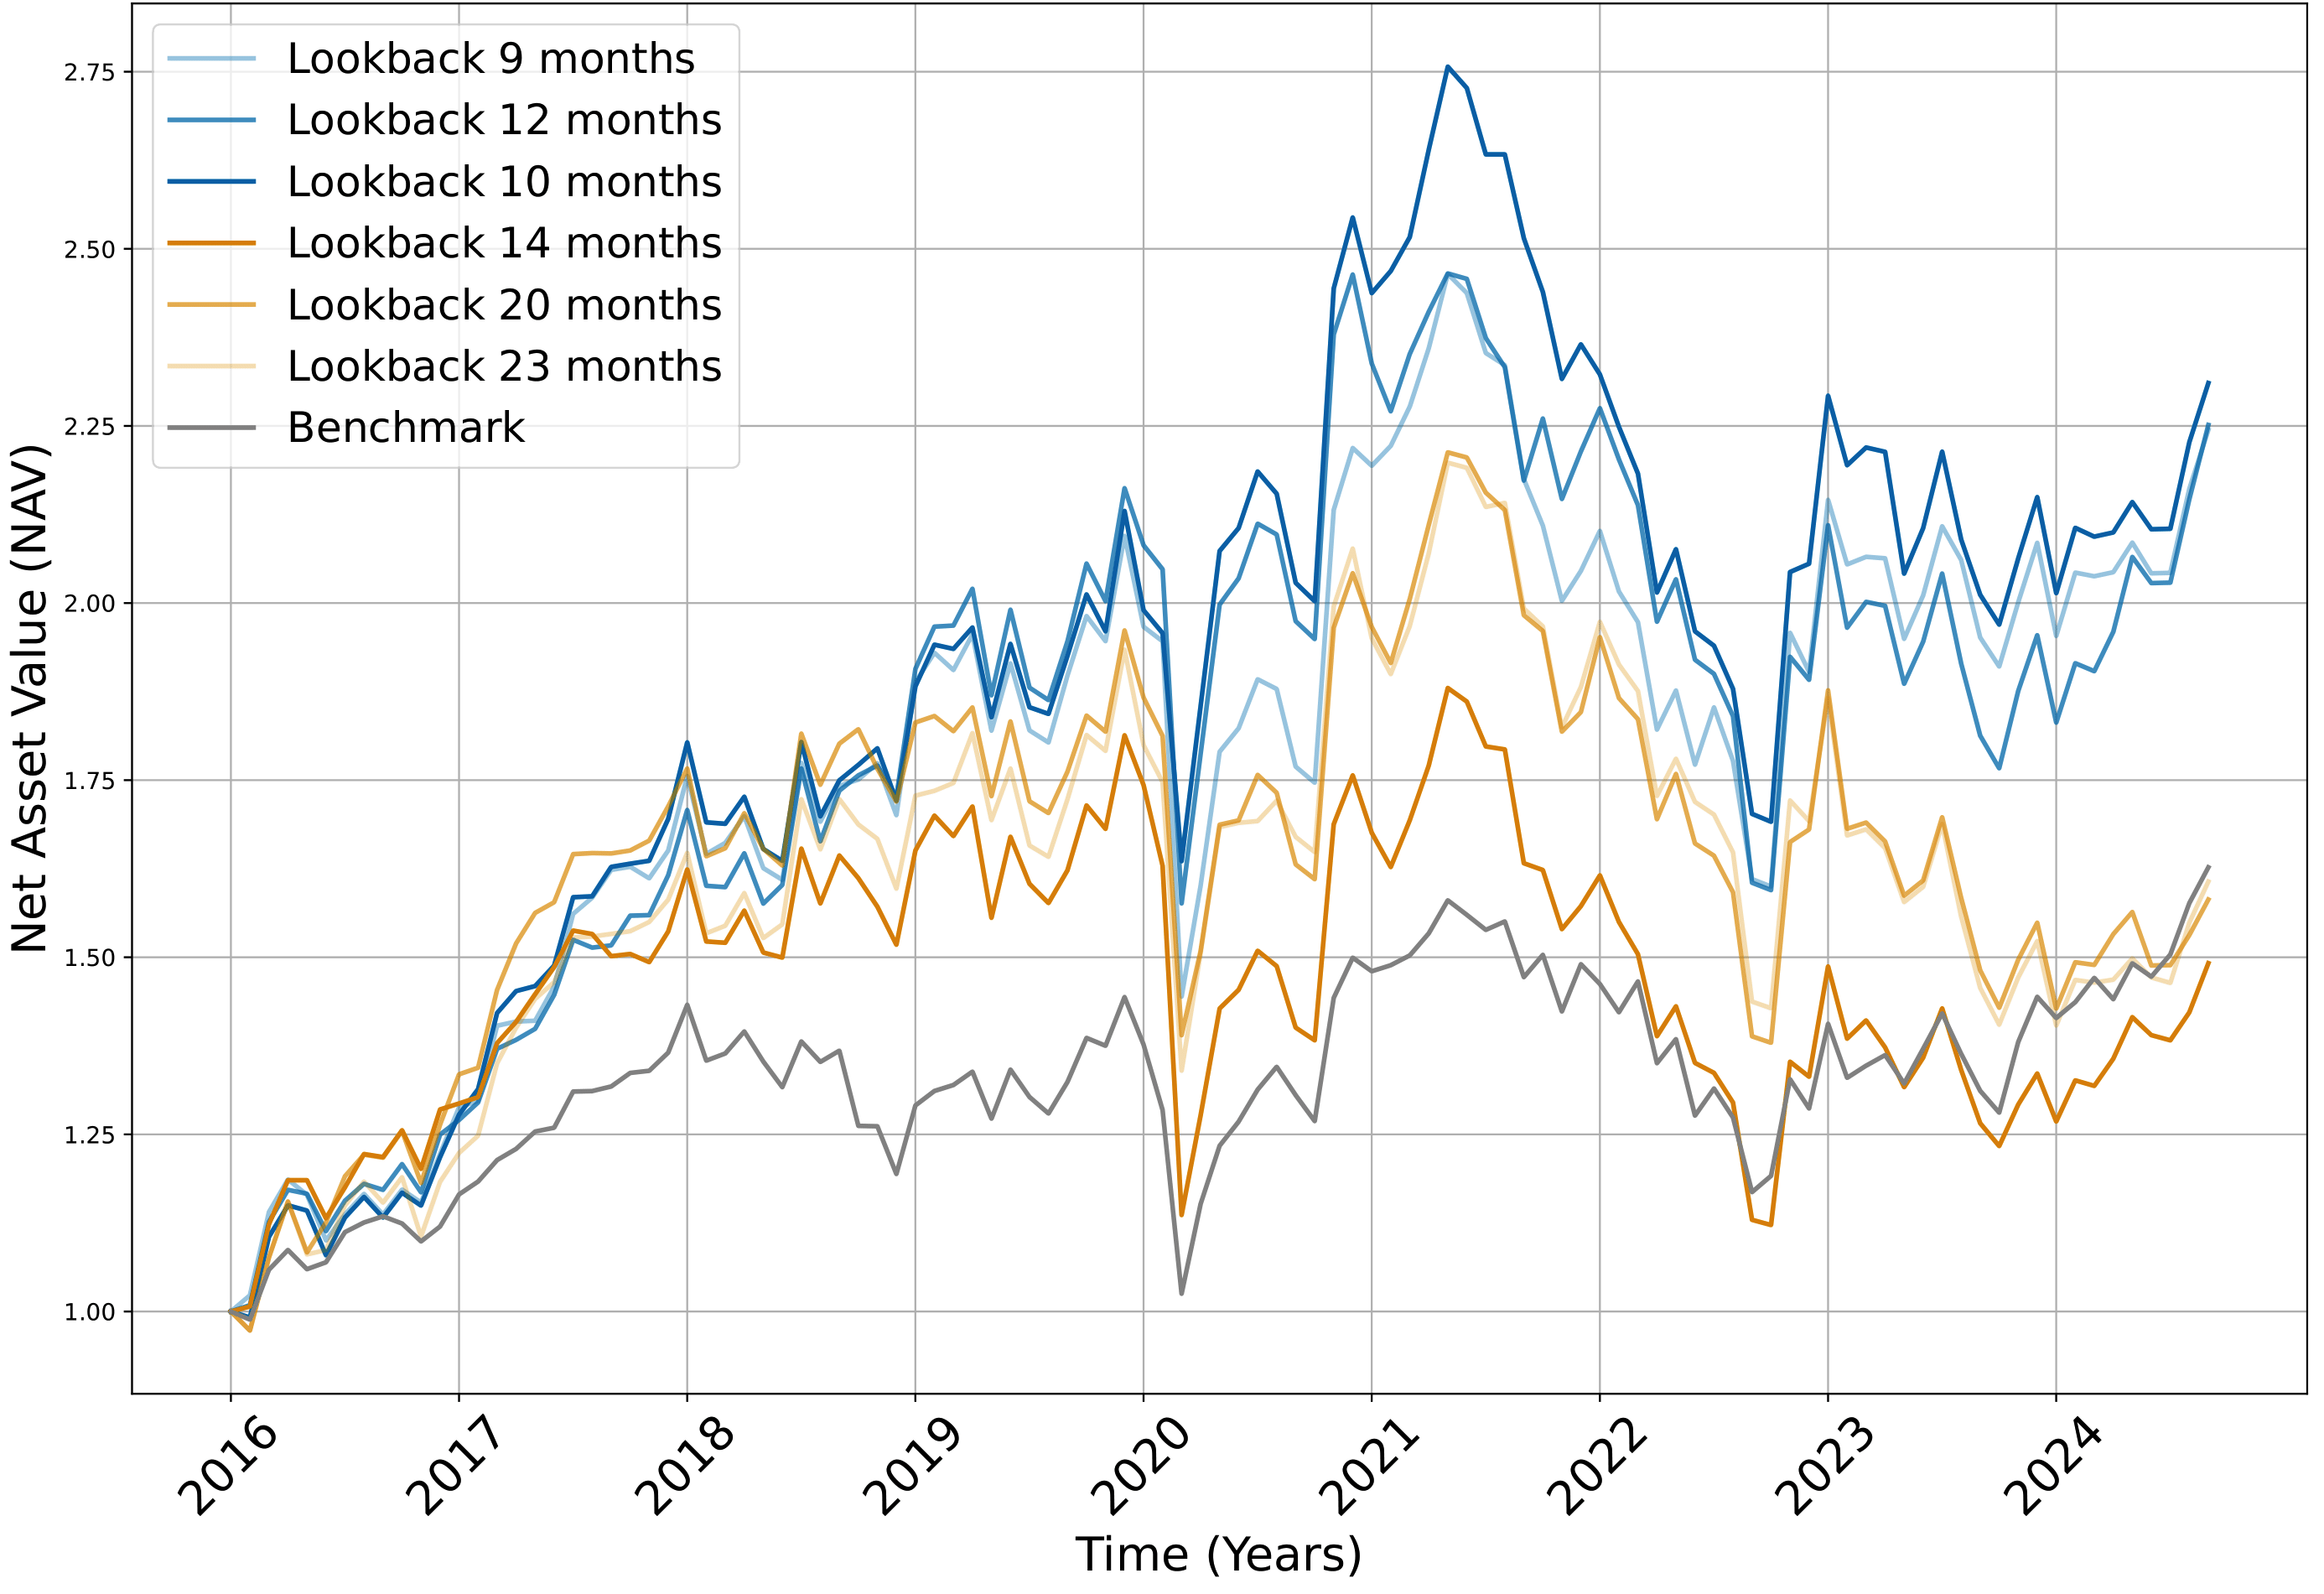
\includegraphics[width=16cm]{figures/fig_bm.png}
    \caption{placeholder}
    \label{fig:bm}
\end{figure}

\begin{figure}[h]
    \centering
    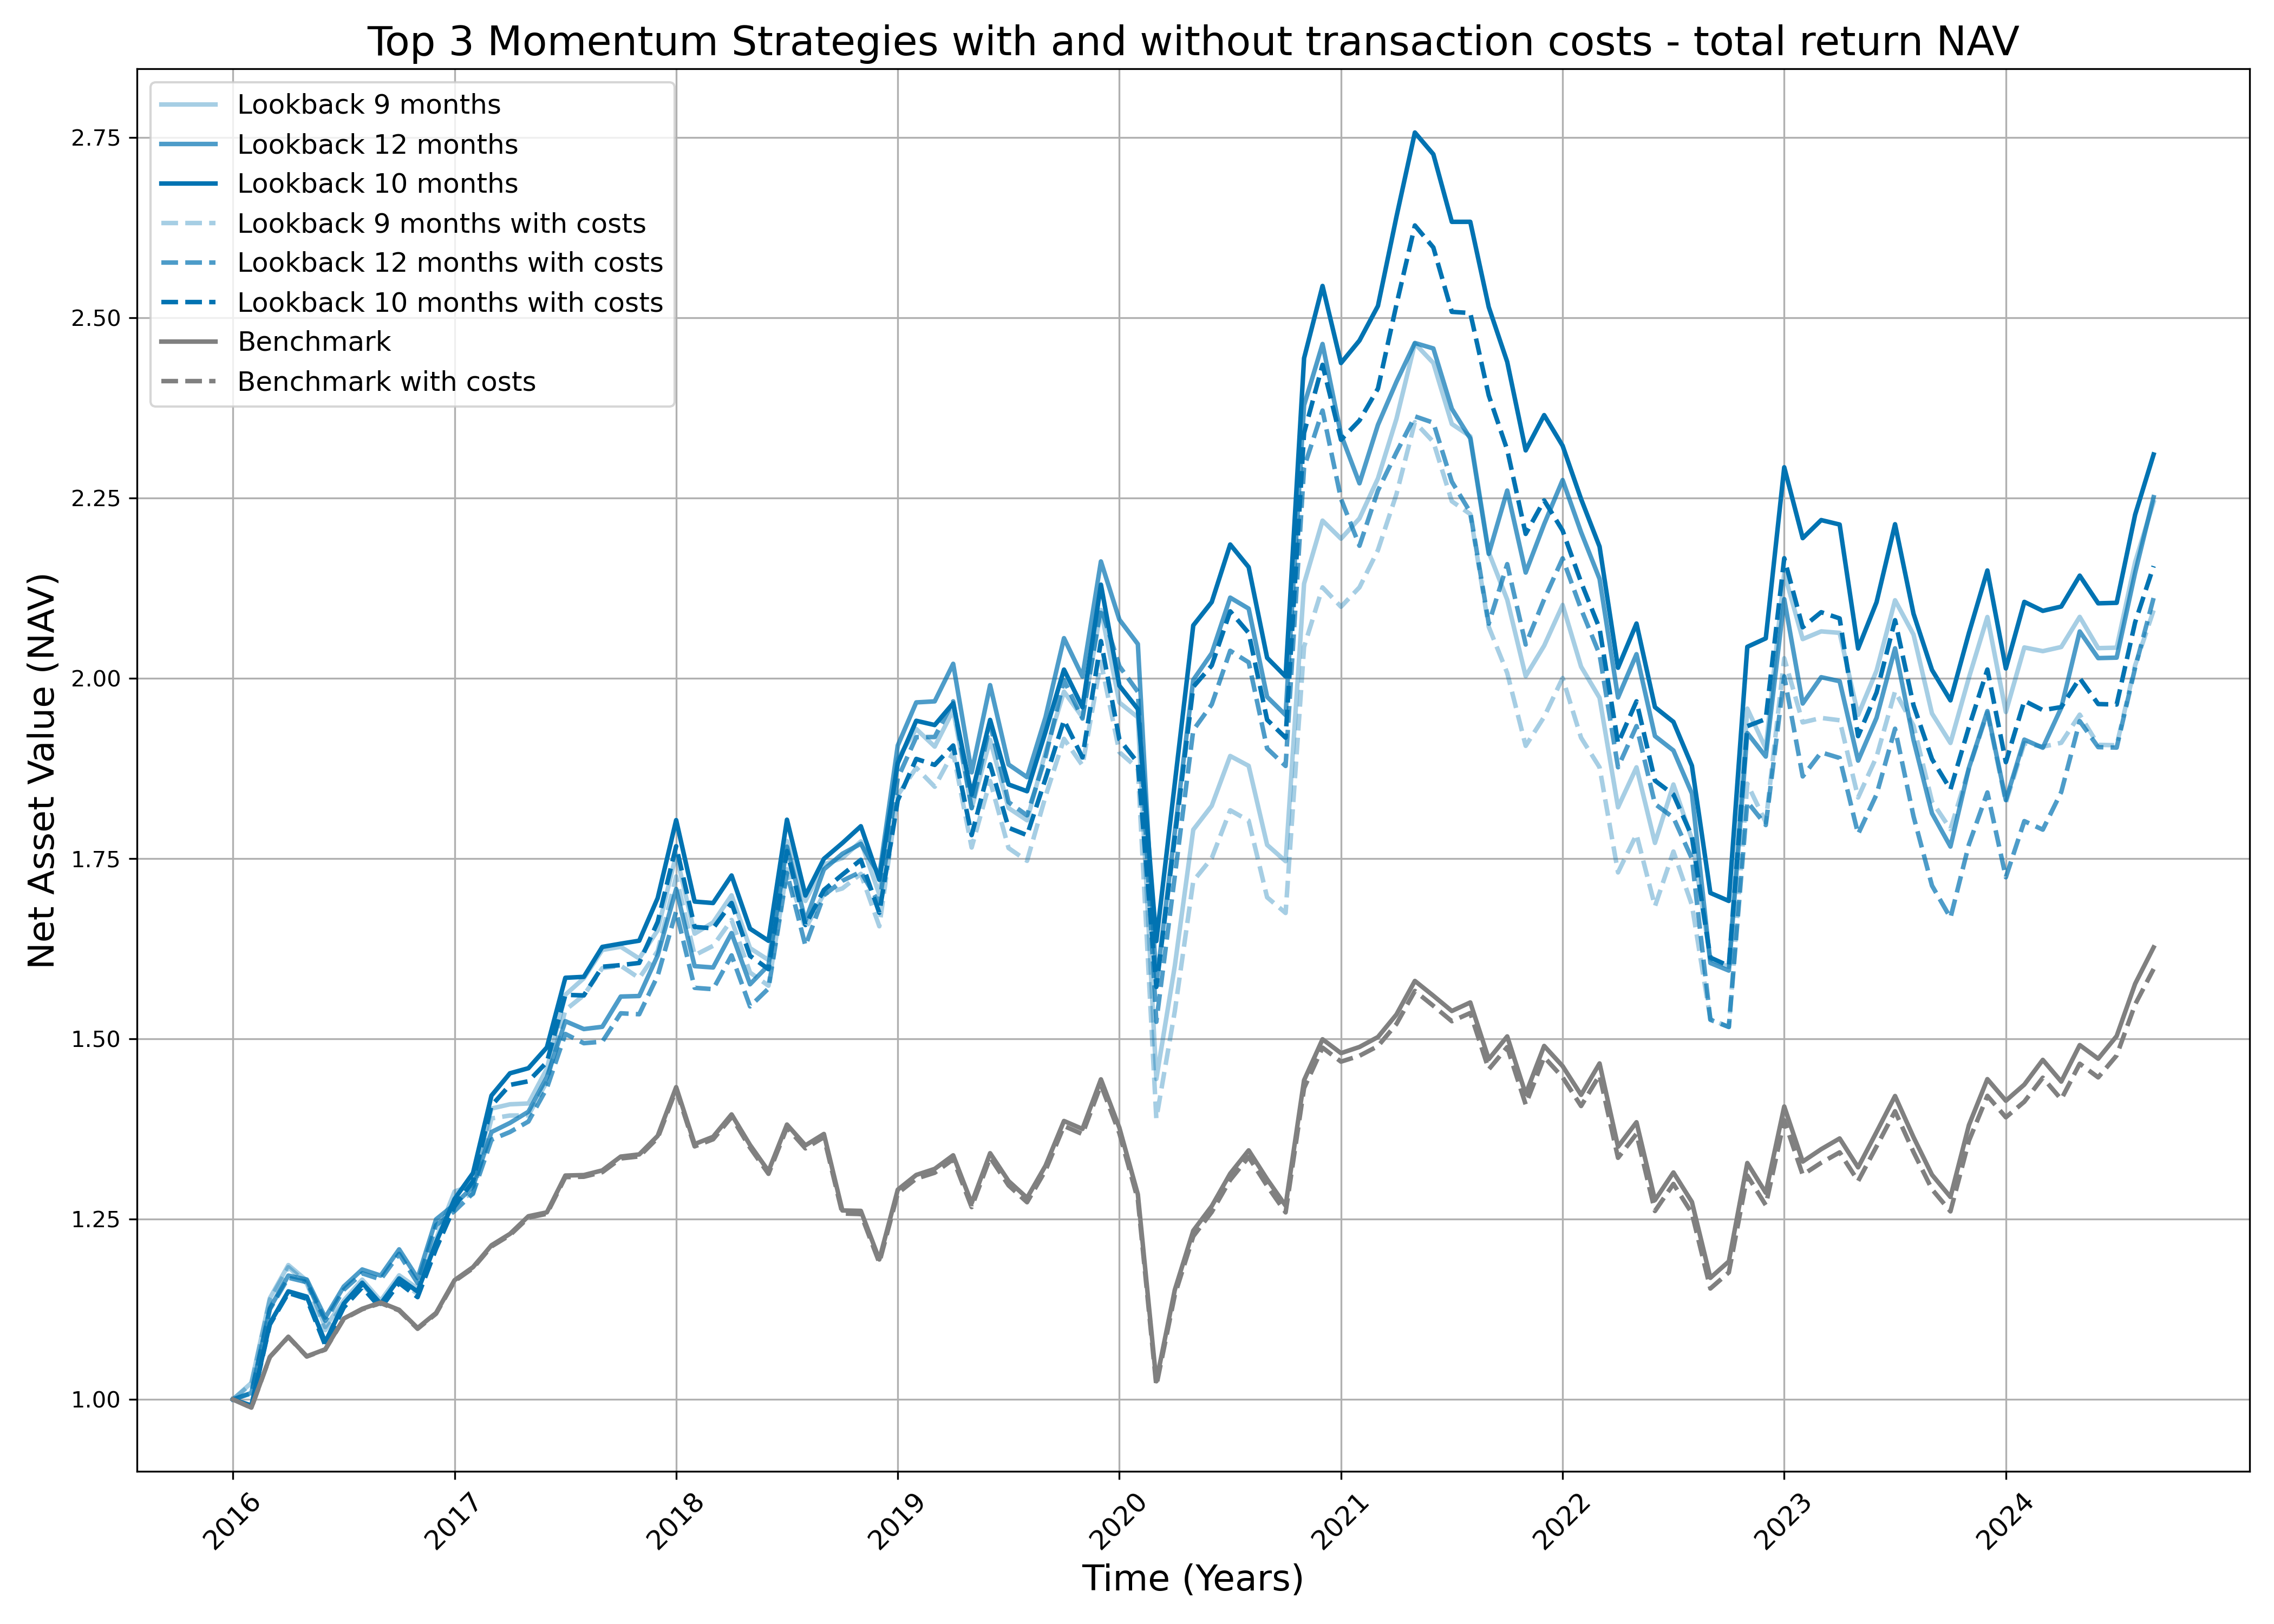
\includegraphics[width=16cm]{figures/fig_costs.png}
    \caption{placeholder}
    \label{fig:costs}
\end{figure}



\clearpage
\newpage
\section{Conclusion}


\clearpage
\bibliographystyle{plainnat}
\bibliography{references}
	
	
\end{document}
